




\chapter{Recurrent Neural Networks}

\section{Introduction}
\noindent Consider the following situation: You are writing an email and you want to do an auto-complete. In this scenario the input would be an incomplete sentence and the output would be the next word in the sentence.\\
\\For example, let the input be:"How are". The answer/output of the auto-complete would be: "you". \\


\noindent A feedforward neural network is not good at solving this kind of problem. The reason is feedforward neural networks can only take fixed-sized inputs, however, a sequence can come in any length so the same network needs to be able to process any input length. Also, since sequences come in varying lengths, parameters need to be shared across each cell, a property a neural network would not support. In an RNN, the parameters in each cell are shared across the number of cells.   \\

\subsection{What is an RNN?} 
 An RNN is a type of artificial neural network using sequential data for problems such as language translation, speech recognition, image captioning, etc. They are different from feedforward neural networks with their "memory" cells as information stored from previous inputs which also influences the current input and the output.  \\

\underline{State System:} Consider a dynamical system of the form:\\
\centerline{\\$\vh_t = f(\vh_{t-1}; \theta$ for $t \geq 1, (h_0 $ given)}
~\\ where 

- $h_t$ is the hidden state at time $t$

- $f: \R^{k} \times \R^{m}$    (Borel Measureable)

- $\theta $ is a parameter of $f$ and is independent of $t$ \\ \\ \\ \\ \\

\begin{example} 
Let $f(x,\theta) = \sigma(\theta x),  \theta \in \R,  |\theta| < 1$.
Consider $\theta=0.5$:
\begin{align*}
    h_0&=2\\
    h_1 &= \sigma(1) \approx 0.73\\
    h_2 &= \sigma(0.73 \times 0.5 ) \approx 0.59\\
    &\vdots\\
    h_{100} &= 0.5708 \ldots
\end{align*}
The reader can check that this converges to approximately $0.5708$ and that this is surprisingly true for any value of $h_0$.
\end{example} 
% .i.e. $H^{(l)}$ and $K^{(l)}$ has size $\frac{H^{(l-1)}-h}{a}+1$ and $\frac{K^{(l-1)}-k}{a}+1$ respectively.
\subsection{Representing a dynamical state system graphically} A dynamical system can be driven by an external signal $X_t$. The values of X could be the words in a sentence and can be represented by the following statement:
$$\vh_t=f(\vh_{t-1}, X_t; \theta)$$
There are two ways to "graph" a dynamical system, the unfolded diagram on the right and the circuit diagram on the left. The circuit diagram is essentially a compressed version of the unfolded diagram.

\begin{figure}[H]
    \centering
    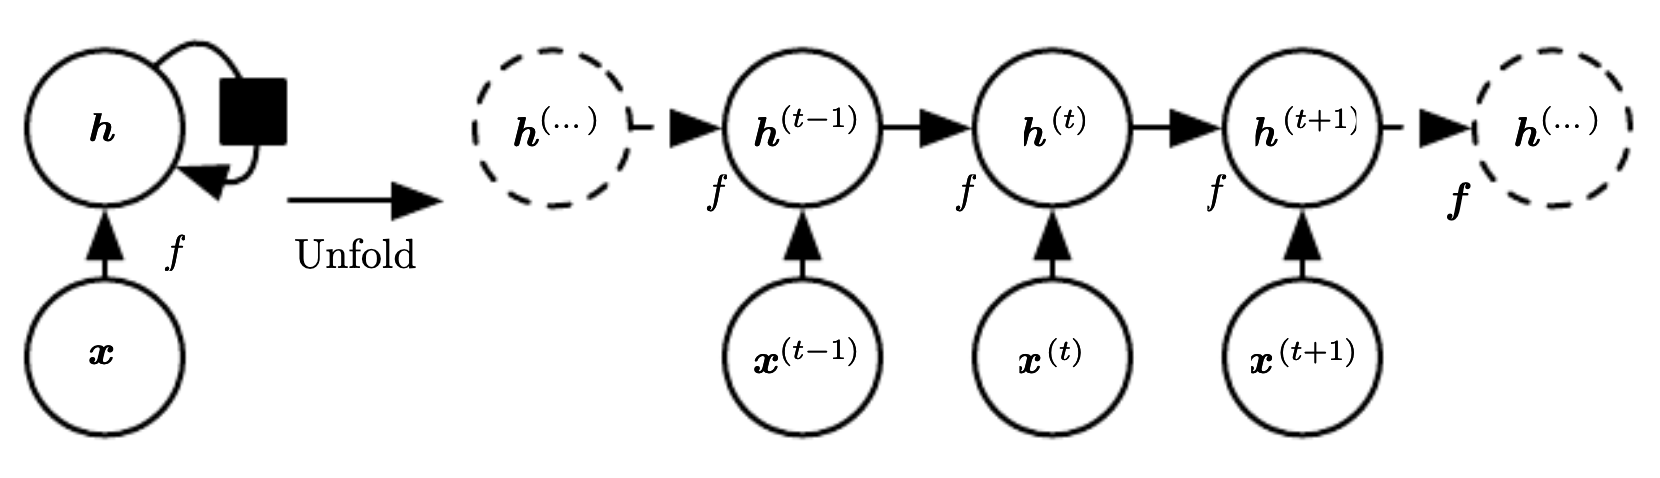
\includegraphics[scale=0.25]{images/Chapter12/circuit_and_unfolded_diagram.png}
    \caption{Circuit diagram (left) and Unfolded diagram (right) are two equivalent ways to represent a Recurrent Neural Network. At each time step ($\blacksquare$), input x is incorporated into state h such that the next state h is influenced by both the current x input and previous x inputs.}
    \label{fig:12.1}
\end{figure}

\section{Recurrent Neural Networks (RNNs)}

An RNN is a state system $(h_{t-1}, X_t; \theta)$ together with a presented way to associate an output $Y_t$ at each time step $(t>0)$.

~\\\underline{Notation:}

- $h_t:$ Hidden State

- $X_t: t^{th}$ input 

- $Y_t: t^th$ output

~\\\underline{Standard Equations}

$$h_t = tanh(Wh_{t-1} + UX_{t} + b)$$
$$Y_t = Vh_t + C$$
$$\theta = (\MW, \MU, \vb,\vc)$$

~\\ where

- $\MW=$ hidden-to-hidden parameters

- $\MU=$ input-to-hidden parameters

- $ \MV=$ hidden-to-output parameters (fixed)

- $\vb,\vc =$ bias vectors

\noindent We can also think of an RNN as a sequence of ordinary feed-forward Neural Networks each with one hidden layer as displayed by the following image:

\begin{center}
$\begin{pmatrix}
 h_0\\
 X_1
\end{pmatrix} \longrightarrow	h_1 \longrightarrow	Y_1$\\
$\begin{pmatrix}
 h_1\\
 X_2
\end{pmatrix} \longrightarrow	h_2 \longrightarrow	Y_2$\\
  $\vdots$
\end{center}
\subsection{Loss Function}
How do we actually apply a loss function to an RNN? Consider an RNN with inputs $x_{1}...x_{T}$ and outputs $y_{1}...y_{T}$ and let's consider a target $z_{1}...z_{T}$ \\

A common choice for the loss function is 

$$ L \left[ \left( y_{1}...y_{T} \right), \left( z_{1}...z_{T} \right) \right] = \sum_{t=1}^{T} \frac{1}{2} \lVert y_{t} - z_{t} \rVert_{2}^2 $$

but one can also use Cross Entropy Loss, Binary Cross Entropy Loss, etc., depending on the situation and context. The loss function would be applied to each state and added up for the total loss.

% $$G \left[ \left( \sum_{s,p}Z^{(l)}_{i+p,j+s,c,f_{\text{in}}} W_{p,s,c,(f_{\text{in}},f_{\text{out}})}^{(l)} \right) + b^{(l)}_{i,j,c,(f_{\text{in}},f_{\text{out}})}\right].$$


\begin{figure}[H]
    \centering
    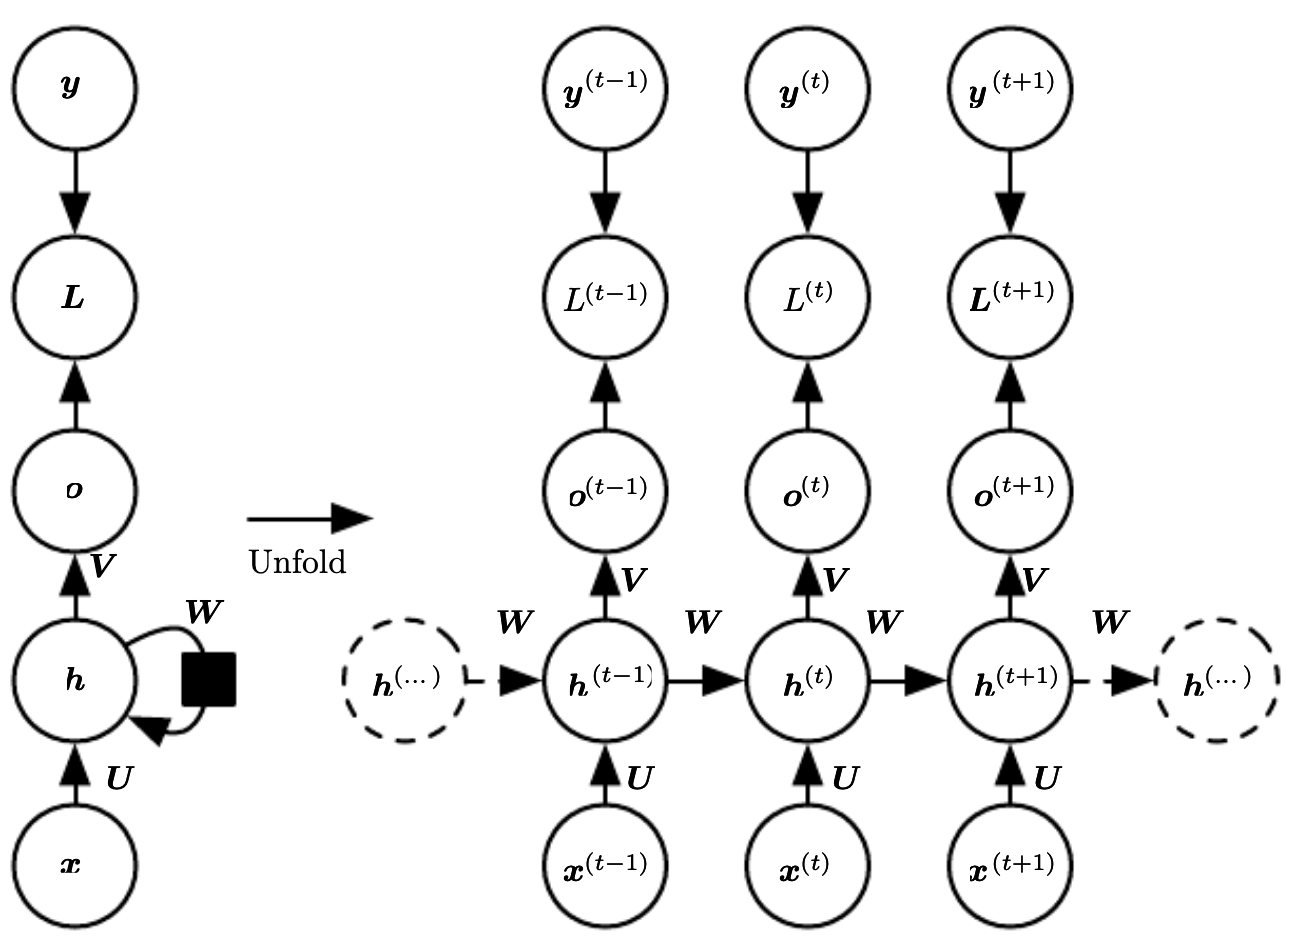
\includegraphics[scale=0.25]{images/Chapter12/RNN_with_loss.png}
    \caption{Loss is calculated between the true y values and the RNN predicted o values at each time step. If one wants a single output from the RNN, the loss can be calculated only between the last y and o values in the sequence.} 
    \label{fig-rnn-loss}
\end{figure}

\begin{example}
    Given a restaurant review, classify if the review is positive or negative.\\
    Review: "It was great"
\end{example}

The RNN will take each of the words as input simultaneously and outputs a binary prediction of positive or negative. 





\begin{figure}[H]
    \centering
    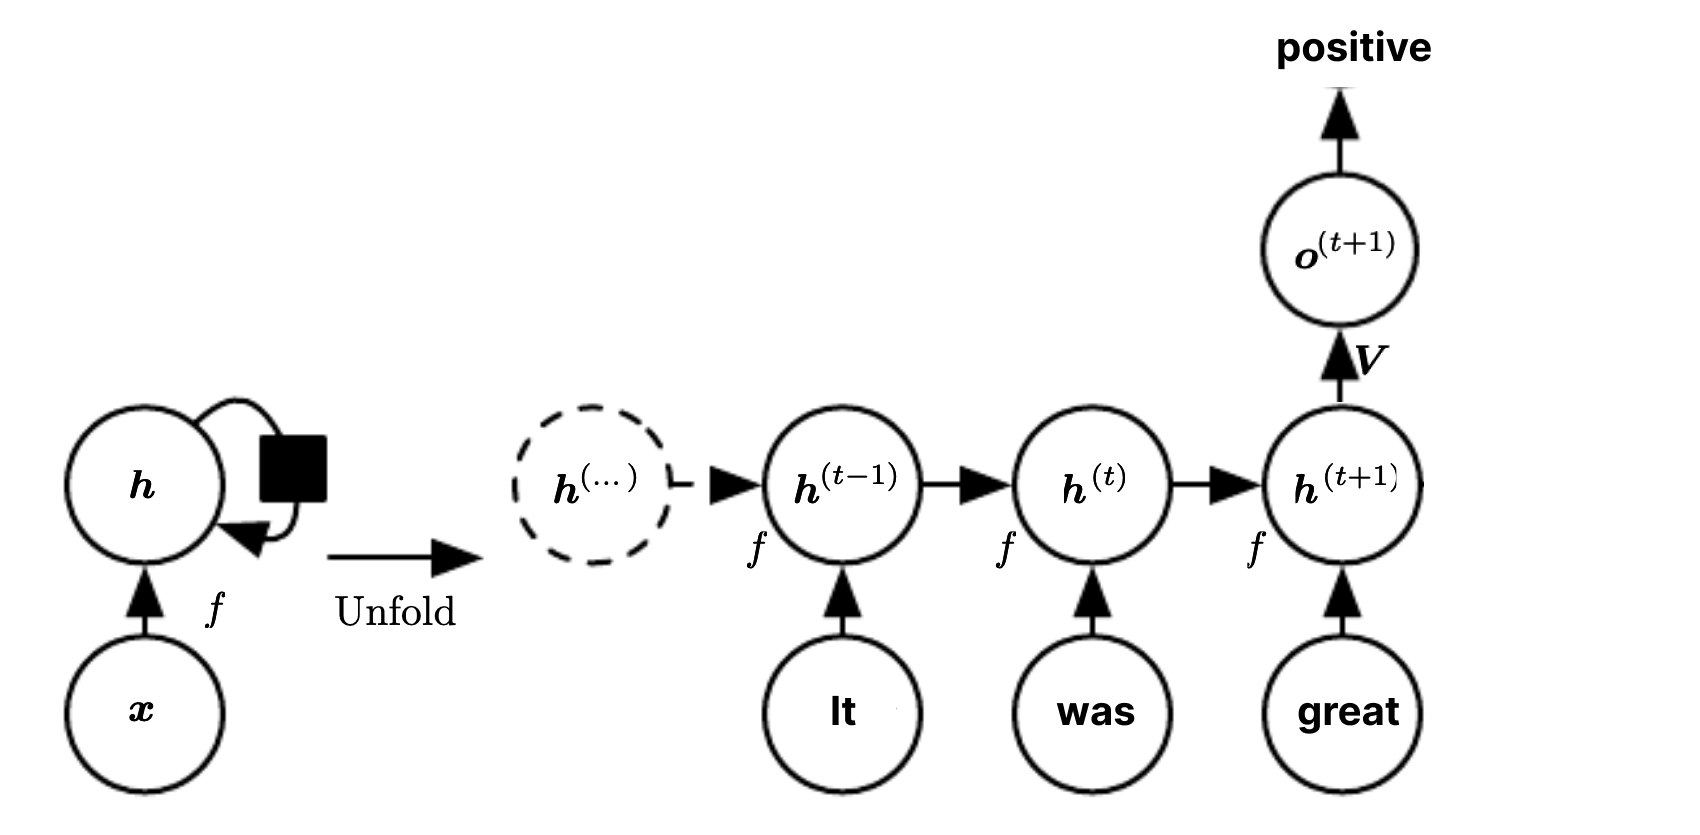
\includegraphics[scale=0.25]{images/Chapter12/sentiment_analysis.png}
    \caption{Given the sequence of words, the RNN makes a binary prediction of positive or negative.}
    \label{fig-rnn}
\end{figure}


\section{RNN backpropagation}
Now, we will be looking at RNN Back-propagation, which is called back propagation through time, where the gradients goes backward at each time steps. One can unroll the computational graph easily by applying the generalized back-propagation algorithm.

\begin{example}
consider an RNN with 2 steps:

\begin{figure}[H]
\centering
  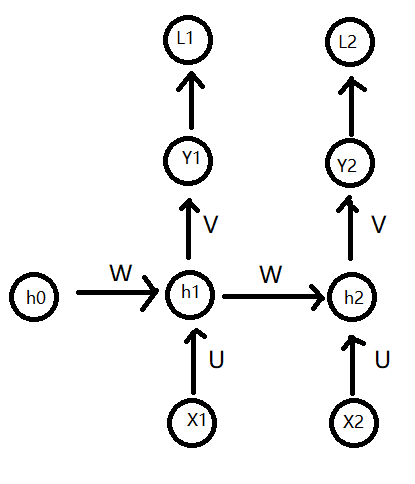
\includegraphics[width=0.35\textwidth]{images/Chapter12/RNNbackprograph.png}
\end{figure}

Where 
\begin{align*}
    a_1=Wh_0+UX_1+b\\
    a_2=Wh_1+UX_2+b\\
    h_1=tanh(a_1)\\
    h_2=tanh(a_2)\\
    Y_1=Vh_1+c\\
    Y_2=Vh_2+c
\end{align*}

using square error loss
\begin{align*}
L=\frac{1}{2}(Y_1-Z_1)^2+\frac{1}{2}(Y_2-Z_2)^2=L_1+L_2
\end{align*}
We want to compute
\begin{align*}
\nabla_\theta L=(\frac{\partial L}{\partial W},\frac{\partial L}{\partial V},\frac{\partial L}{\partial U},\frac{\partial L}{\partial b},\frac{\partial L}{\partial c})
\end{align*}Note that $L_1$ depends on $W$ only through $h_1$, and $L_2$ depends on $W$ through $h_1$ and $h_2$, so

\begin{align*}
\frac{\partial L}{\partial W}=\frac{\partial L_1}{\partial W}+\frac{\partial L_2}{\partial W}=\frac{\partial L1}{\partial h_1} \frac{\partial h_1}{\partial W}+\frac{\partial L_2}{\partial h_1} \frac{\partial h_1}{\partial W}+\frac{\partial L_2 }{\partial h_2}\frac{\partial h_2}{\partial W} 
\end{align*}

\begin{align*}
\frac{\partial L}{\partial V}=\frac{\partial L_1}{\partial V}+\frac{\partial L_2}{\partial V}=\frac{\partial L_1}{\partial Y_1}\frac{\partial Y_1}{\partial V}+\frac{\partial L_2}{\partial Y_2}\frac{\partial Y_2}{\partial V} \\
\Rightarrow \frac{\partial L}{\partial V}=(Y_1-Z_1)h_1+(Y_2-Z_x)h_2=\sum_{t}(Y_t-Z_t)h_t\\
\end{align*}

\begin{align*}
\frac{\partial L}{\partial U}=\frac{\partial L_1}{\partial U}+\frac{\partial L_2}{\partial U}=\frac{\partial L_1}{\partial h_1}\frac{\partial h_1}{\partial U}+\frac{\partial L_2}{\partial h_1}\frac{\partial h_1}{\partial U}+\frac{\partial L_2}{\partial h_2}\frac{\partial h_2}{\partial U}\\
\Rightarrow \frac{\partial L}{\partial U}=\frac{\partial L_1}{\partial h_1}\frac{\partial h_1}{\partial U}+\frac{\partial L_2}{\partial h_2}\frac{\partial h_2}{\partial h_1}\frac{\partial h_1}{\partial U}+\frac{\partial L_2}{\partial h_2}\frac{\partial h_2}{\partial U}\\
\end{align*}

\begin{align*}
\frac{\partial L}{\partial b}=\frac{\partial L_1}{\partial b}+\frac{\partial L_2}{\partial b}=\frac{\partial L_1}{\partial h_1}\frac{\partial h_1}{\partial b}+\frac{\partial L_2}{\partial h_1}\frac{\partial h_1}{\partial b}+\frac{\partial L_2}{\partial h_2}\frac{\partial h_2}{\partial b}\\
\Rightarrow \frac{\partial L}{\partial b}= \frac{\partial L_1}{\partial h_1}\frac{\partial h_1}{\partial b}+\frac{\partial L_2}{\partial h_2}\frac{\partial h_2}{\partial h_1}\frac{\partial h_1}{\partial b}+\frac{\partial L_2}{\partial h_2}\frac{\partial h_2}{\partial b}
\end{align*}

\begin{align*}
\frac{\partial L}{\partial c}=\frac{\partial L_1}{\partial c}+\frac{\partial L_2}{\partial c}=\frac{\partial L_1}{\partial Y_1}\frac{\partial Y_1}{\partial c}+\frac{\partial L_2}{\partial Y_2}\frac{\partial Y_2}{\partial c}\\
\Rightarrow \frac{\partial L}{\partial c}=(Y_1-Z_1)+(Y_2-Z_2)=\sum_{t}(Y_t-Z_t)
\end{align*}



With the above computed, it is suffice to compute the following:

\begin{align*}
\frac{\partial L_1}{\partial h_1}=\frac{\partial L_1}{\partial Y_1}\frac{\partial Y_1}{\partial h_1}=(Y_1-Z_1)V\\[1em]
\frac{\partial L_2}{\partial h_2}=\frac{\partial L_2}{\partial Y_2}\frac{\partial Y_2}{\partial h_2}=(Y_2-Z_2)V\\[1em]
\frac{\partial h_1}{\partial W}=\frac{\partial }{\partial W} \tanh (a_1)=sech^2(a_1)\frac{\partial a_1}{\partial W}\\
=(1-\tanh ^2(a_1))=(1-h_1^2)h_0\\[1em]
\frac{\partial h_2}{\partial W}=\frac{\partial }{\partial W} \tanh (a_2)=sech^2(a_2)\frac{\partial a_2}{\partial W}\\
=(1-\tanh ^2(a_2))=(1-h_2^2)h_1\\[1em]
\frac{\partial h_2}{\partial h_1}=\frac{\partial }{\partial h_1} \tanh (a_2)=sech^2(a_2)\frac{\partial a_2}{\partial h_1}=(1-h_2^2)W\\[1em]
\frac{\partial h_1}{\partial U}=\frac{\partial }{\partial U} \tanh (a_1)=(1-h_1^2)\frac{\partial a_1}{\partial U}=(1-h_1^2)X_1\\[1em]
\frac{\partial h_2}{\partial U}=\frac{\partial }{\partial U} \tanh (a_2)=(1-h_2^2)\frac{\partial a_2}{\partial U}=(1-h_2^2)X_2\\[1em]
\frac{\partial h_1}{\partial b}=\frac{\partial }{\partial b}\tanh (a_1)=sech^2(a_1)\frac{\partial a_1}{\partial b}=(1-h_1^2)\\[1em]
\frac{\partial h_2}{\partial b}=\frac{\partial }{\partial b}\tanh (a_2)=sech^2(a_2)\frac{\partial a_2}{\partial b}=(1-h_2^2)
\end{align*}
\end{example}

\section{Exercises}
\begin{enumerate}
    \item What are Recurrent Neural Networks (RNN) used for and why can't we just use a Neural Network?
            
    \item How is Loss calculated in an RNN?
    
    \item Write an algorithm or pseudocode to model a state system with inputs hidden state $h_0$, $\theta$, and time step T to indicate the number of iterations where $f(x,\theta) = \sigma(\theta x), \theta \in \R,  |\theta| < 1$.\\
    
      
\end{enumerate}



\section{Solutions to Exercises}

\begin{enumerate}
    \item  A feedforward neural network is not good at solving this kind of problem because it only can take a fixed length as input, however, a sequence has varying lengths. We need a model that is specialized in learning sequential dependencies between values in the sequence. An RNN is used for processing and handling chunks of a sequence.

    \item  Loss is calculated by summing each individual loss at each time step. The loss function is applied to each actual y value and the output of each cell.  

    \item Here is the pseudocode function for stateSystem.\\

    \begin{algorithm}
    \caption{$stateSystem(\textbf{h},theta, T)$}
    \begin{algorithmic}[1]
        \State i = 0
        \State def stateSystem(h, theta, T):
            \State \indent h = h * theta
            \State \indent if $i == T$ then
		\State  \indent \indent return h
            
	\end{algorithmic} 
\end{algorithm}
   


\end{enumerate}